43. а) $f(x)=|x^2-2x|=\begin{cases} x^2-2x,\ x\leqslant 0,\\ 2x-x^2,\ 0<x<2,\\ x^2-2x,\ x\geqslant2.\end{cases}$
$$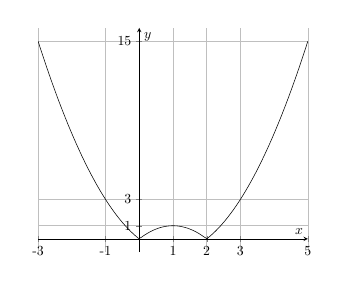
\begin{tikzpicture}[scale=0.5]
\begin{axis}[
    axis lines = middle,
    grid=major,
    legend pos={south west},
    xlabel = {$x$},
    %xlabel style={below right},
    ylabel = {$y$},
    ymin=-1,
    ymax=16,
    xmin=-3,
    xmax=5,
    xtick={-3,-1,1,2,3,5,7},
    xticklabels={-3,-1,1,2,3,5,7},
    ytick={ 15,3,1},
    yticklabels={ 15,3,1},
                  ]
	\addplot[domain=-3:5, samples=100, color=black] {abs(x*x-2*x)};
   % \addplot[domain=-3:3, samples=100, color=black] {-x};
     %\addlegendentry{$\text{Рис. 1}$};
\end{axis}
\end{tikzpicture}$$
б) По графику определим количество решений: $a\in(-\infty;0):0,\ a\in\{0\}\cup(1;+\infty):2,\ a=1: 3,$\\$ a\in(0;1): 4.$\\
